\documentclass[tikz, preview]{standalone}

\usepackage{amsfonts, amsthm, amssymb, amsmath, stmaryrd, etoolbox}
\usepackage{tikz}
\usepackage[all,2cell]{xy}
\usetikzlibrary{matrix,arrows,shapes,decorations.markings,decorations.pathreplacing}
\definecolor{rewritecolor}{rgb}{0,.9,1}
\tikzset{rewritenode/.style={shape=circle,fill=rewritecolor,scale=0.25,font=\Huge}}
\tikzset{RWopen/.style={shape=circle,draw=black,fill=white,scale=0.5,font=\Huge}}
\tikzset{RWclosed/.style={shape=circle,fill=black,scale=0.5,font=\Huge}}
\tikzset{CDnode/.style={shape=circle,fill=white,scale=.5}}
\tikzset{zxgreen/.style={shape=circle,draw,thick,fill=green}}
\tikzset{zxred/.style={shape=circle,draw,thick,fill=red}}
\tikzset{zxyellow/.style={shape=rectangle,draw,thick,fill=yellow}}
\tikzset{zxdiamond/.style={shape=diamond,fill=black,inner sep=2.75}}
\tikzset{zxopen/.style={shape=circle,draw,thick,inner sep=2pt}}
\tikzset{->-/.style={decoration={markings,mark=at position .5 with {\arrow{>}}},postaction={decorate}}}

\begin{document}
\[
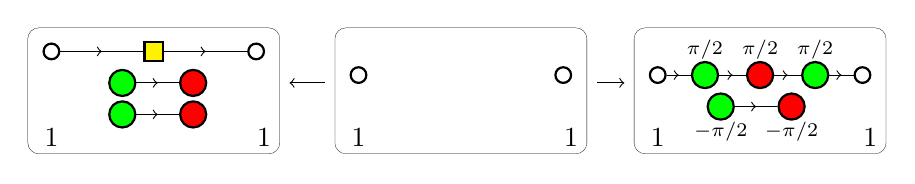
\begin{tikzpicture}
	\begin{scope}[shift={(-3.7,-0.6)}]
	\node [zxopen] (v1) at (-0.6,0.4) {};
	\node [zxgreen] (v2) at (0.3,0) {};
	\node [zxgreen] (v3) at (0.3,-0.4) {};
	\node [zxred] (v4) at (1.2,0) {};
	\node [zxred] (v5) at (1.2,-0.4) {};
	\node [zxopen] (v6) at (2,0.4) {};
	\node [zxyellow] (v7) at (0.7,0.4) {};
	%
	\draw [->-] (v1) to (v7);
	\draw [->-] (v7) to (v6);
	\draw [->-] (v2) to (v4);
	\draw [->-] (v3) to (v5);
	%
	\node at (-0.6,-0.7) {$1$};
	\node at (2.1,-0.7) {$1$};
	\node (v11) at (2.3,0) {};
	\draw [ultra thin, rounded corners] (-0.9,0.7) rectangle (2.3,-0.9);
	\end{scope}
	%
	%
	%
	\begin{scope}[shift={(2.3,-0.1)}]
	\node [zxopen] (v1) at (-2.7,-0.4) {};
	\node [zxopen] (v2) at (-0.1,-0.4) {};
	%
	\draw [ultra thin, rounded corners] (-3,0.2) rectangle (0.2,-1.4);
	\node at (-2.7,-1.2) {$1$};
	\node at (0,-1.2) {$1$};
	\node (v12) at (-3,-0.5) {};
	\node (v14) at (0.2,-0.5) {};
	\end{scope}
	%
	%
	%
	\begin{scope}[shift={(5.1,-0.5)}]
	\node [zxopen] (v8) at (-1.7,0) {};
	\node [zxgreen,label={[shift={(0,-0.1)}]\scriptsize $\pi/2$}] (v9) at (-1.1,0) {};
	\node [zxred,label={[shift={(0,-0.1)}]\scriptsize $\pi/2$}] (v10) at (-0.4,0) {};
	\node [zxgreen,label={[shift={(0,-0.1)}]\scriptsize $\pi/2$}] (v15) at (0.3,0) {};
	\node [zxopen] (v16) at (0.9,0) {};
	\node [zxgreen,label={[shift={(0,-0.75)}]\scriptsize $-\pi/2$}] (v17) at (-0.9,-0.4) {};
	\node [zxred,label={[shift={(0,-0.75)}]\scriptsize $-\pi/2$}] (v18) at (0,-0.4) {};
	%
	\node at (-1.7,-0.8) {$1$};
	\node at (1,-0.8) {$1$};
	\draw [ultra thin, rounded corners] (-2,0.6) rectangle (1.2,-1);
	\node (v13) at (-2,-0.1) {};
	%
	\draw [->-] (v8) to (v9);
	\draw [->-] (v9) to (v10);
	\draw [->-] (v10) to (v15);
	\draw [->-] (v15) to (v16);
	\draw [->-] (v17) to (v18);
	\end{scope}
	%
	%
	%
	\draw [<-] (v11) edge (v12);
	\draw [<-] (v13) edge (v14);
\end{tikzpicture}
\]
\end{document}
